\documentclass[tikz]{standalone}
\usepackage{tikz}

\begin{document}
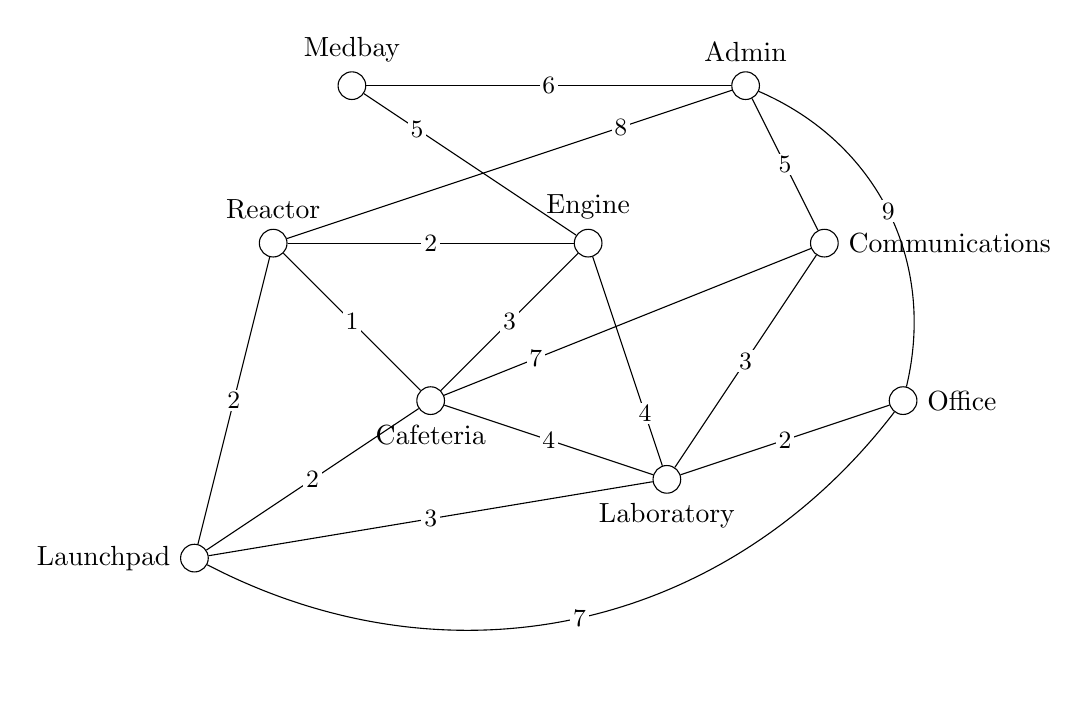
\begin{tikzpicture}
    [mynode/.style={draw, circle, inner sep = 0em, minimum size = 10},
     edgelabel/.style = {fill = white, inner sep = 1, font=\small}]

    % nodes inside the curve
    \node[mynode, label=180:{Launchpad}] (Launchpad) at (-3, -2) {};
    \node[mynode, label=90:{Reactor}] (Reactor) at (-2, 2) {};
    \node[mynode, label=270:{Laboratory}] (Laboratory) at (3, -1) {};
    \node[mynode, label=90:{Medbay}] (Medbay) at (-1, 4) {};
    \node[mynode, label=0:{Communications}] (Communications) at (5, 2) {};
    \node[mynode, label=0:{Office}] (Office) at (6, 0) {};
    \node[mynode, label=90:{Admin}] (Admin) at (4, 4) {};
    \node[mynode, label=90:{Engine}] (Engine) at (2, 2) {};
    \node[mynode, label=270:{Cafeteria}] (Cafeteria) at (0, 0) {};

    % % nodes outside of the curve
    % \node[mynode] (d) at (0.5, 1.5) {d};
    % \node[mynode] (e) at (0, 0.5) {e};
    % \node[mynode] (f) at (0.2, -0.8) {f};
    % \node[mynode] (g) at (0.4, -1.9) {g};

    % % edges between inside and outside nodes
    \draw[-] (Launchpad) to node[edgelabel] {$2$} (Cafeteria);
    \draw[-] (Launchpad) to node[edgelabel] {$3$} (Laboratory);
    \draw[-] (Launchpad) to node[edgelabel] {$2$} (Reactor);
    \draw[-, bend right=40] (Launchpad) to node[edgelabel] {$7$} (Office);
    \draw[-] (Laboratory) to node[edgelabel] {$4$} (Cafeteria);
    \draw[-] (Laboratory) to node[edgelabel, near start] {$4$} (Engine);
    \draw[-] (Laboratory) to node[edgelabel] {$3$} (Communications);
    \draw[-] (Laboratory) to node[edgelabel] {$2$} (Office);
    \draw[-] (Cafeteria) to node[edgelabel] {$1$} (Reactor);
    \draw[-] (Cafeteria) to node[edgelabel] {$3$} (Engine);
    \draw[-] (Cafeteria) to node[edgelabel, near start] {$7$} (Communications);
    \draw[-] (Admin) to node[edgelabel] {$5$} (Communications);
    \draw[-] (Admin) to node[edgelabel] {$6$} (Medbay);
    \draw[-, bend left=40] (Admin) to node[edgelabel] {$9$} (Office);
    \draw[-] (Engine) to node[edgelabel, near end] {$5$} (Medbay);
    \draw[-] (Engine) to node[edgelabel] {$2$} (Reactor);
    \draw[-] (Reactor) to node[edgelabel, near end] {$8$} (Admin);
    % \draw[->] (a) to node[edgelabel] {$1$} (e);
    % \draw[->] (a) to node[edgelabel, near start] {$1$} (f);
    % \draw[->] (b) to node[edgelabel] {$1$} (e);
    % \draw[->] (c) to node[edgelabel, near start] {$1$} (e);
    % \draw[->] (c) to node[edgelabel] {$1$} (g);

\end{tikzpicture}
\end{document}